La componente relativa all'unità viene sviluppata utilizzando il run-time \glock{Node.JS} e i \glock{WebSocket} per la comunicazione con le componenti del server e dei sensori, mentre per lo strato di persistenza si é deciso di fare utilizzo del database \glock{MongoDB}.
La scelta architetturale per questa componente é ricaduta sulla \textit{Hexagonal Architecture}.
I motivi riconducibili alla suddetta scelta sono da riscontrarsi nella natura semplicistica del servizio che la componente mette a disposizione. Le logiche di business si occupano unicamente di controllare che i dati ricevuti (già validati nel formato) vengano esaminati e processati per poi essere salvati sul persistence layer.
Il punto fondamentale é che, oltre ai controller, anche la classe \textit{UnitEngine} si occupa di scrivere e leggere dati dallo strato di persistenza, in modo da emulare l'evolvere degli stati mano a mano che l'unità avanza lungo il percorso e/o incontra ostacoli.
É inoltre prevista, similmente a quanto accade per la parte relativa alla UI, una gerarchia di interfacce e classi che si occupano di modellare tutti i possibili messaggi che l'unità può voler scambiare con le altre componenti, in modo da controllare in maniera più pulita il passaggio di informazioni.
Per quanto concerne i sensori, invece, essi non sono dotati di una reale architettura, data la trivialità del loro scopo e del modo in cui il componente opera per raggiungerlo.

\begin{figure}[H]
	\centering
	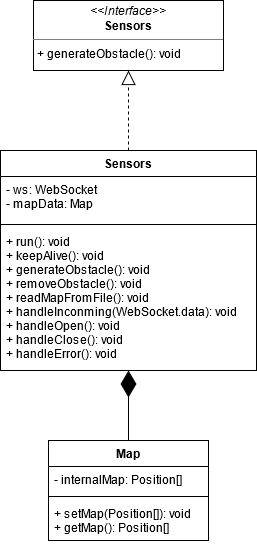
\includegraphics[width=6cm]{img/unit_sensori.png}
	\caption{Unità - Sensori}
\end{figure}

Di seguito si illustrano i diagrammi delle classi dell'architettura dell'unità, e dei messaggi usati per interfacciarsi con il server.

\begin{landscape}
	\begin{figure}[h!]
		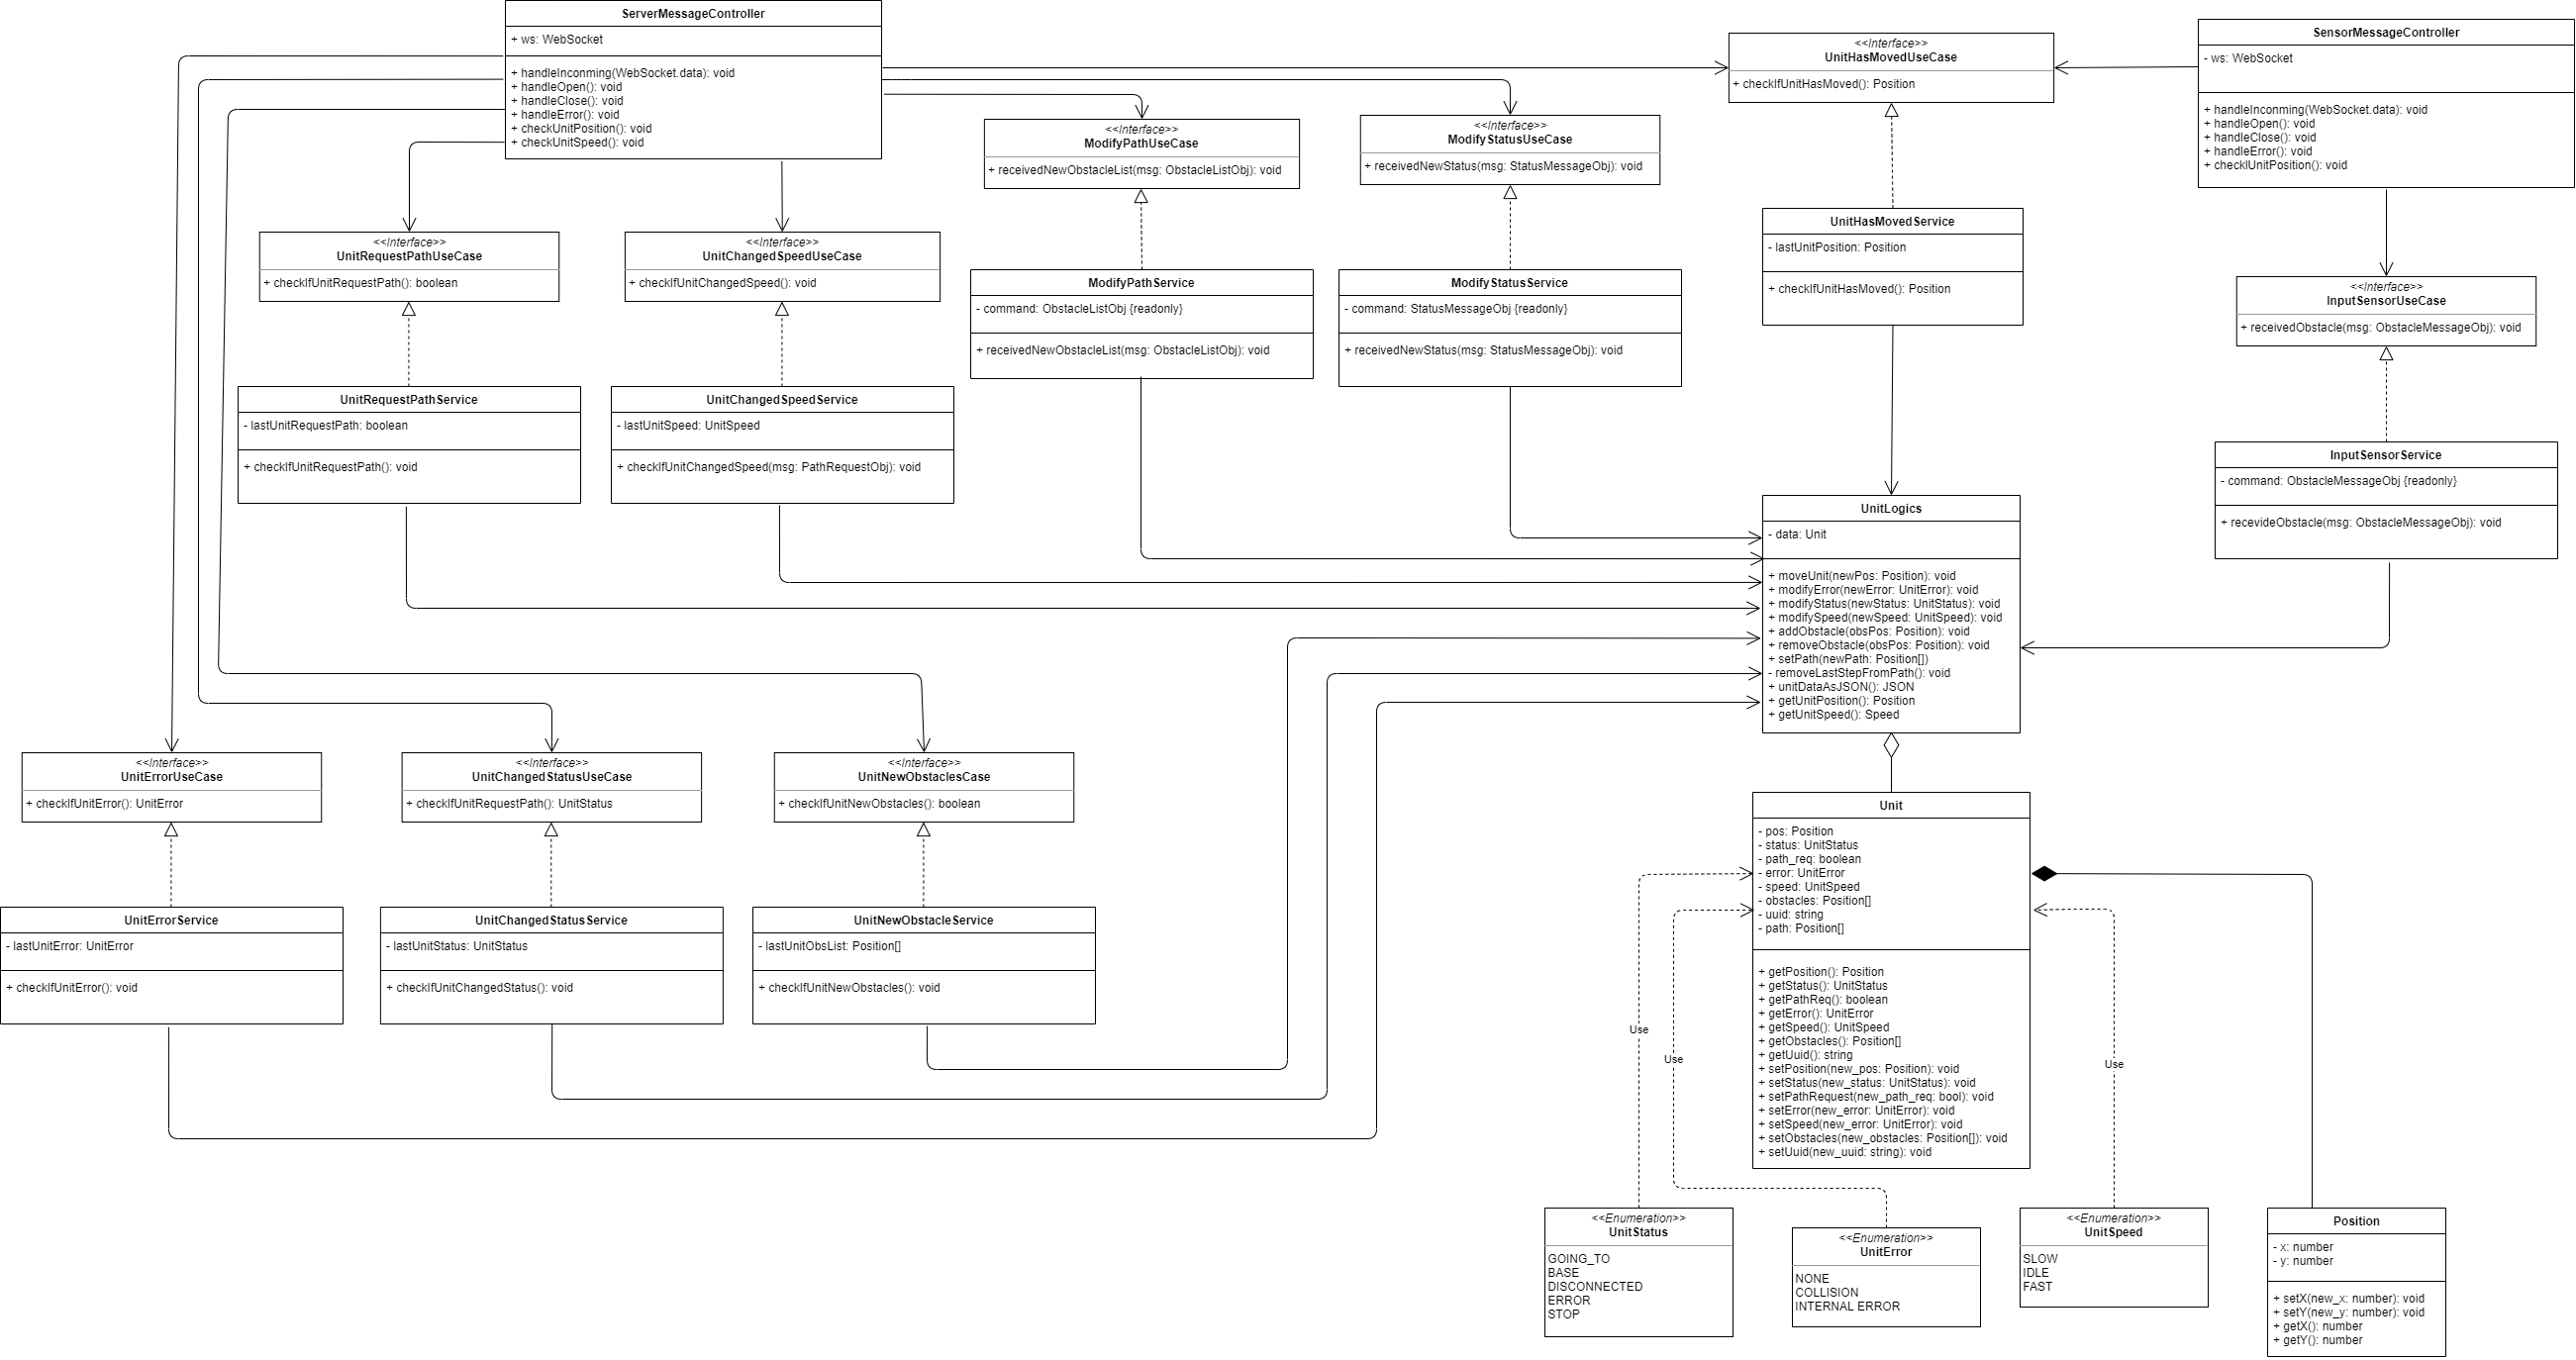
\includegraphics[width=25.5cm]{img/unit_architettura.png}
		\caption{Unità - Diagramma delle classi}
	\end{figure}
\end{landscape}

\begin{landscape}
    \begin{figure}[H]
    	\centering
    	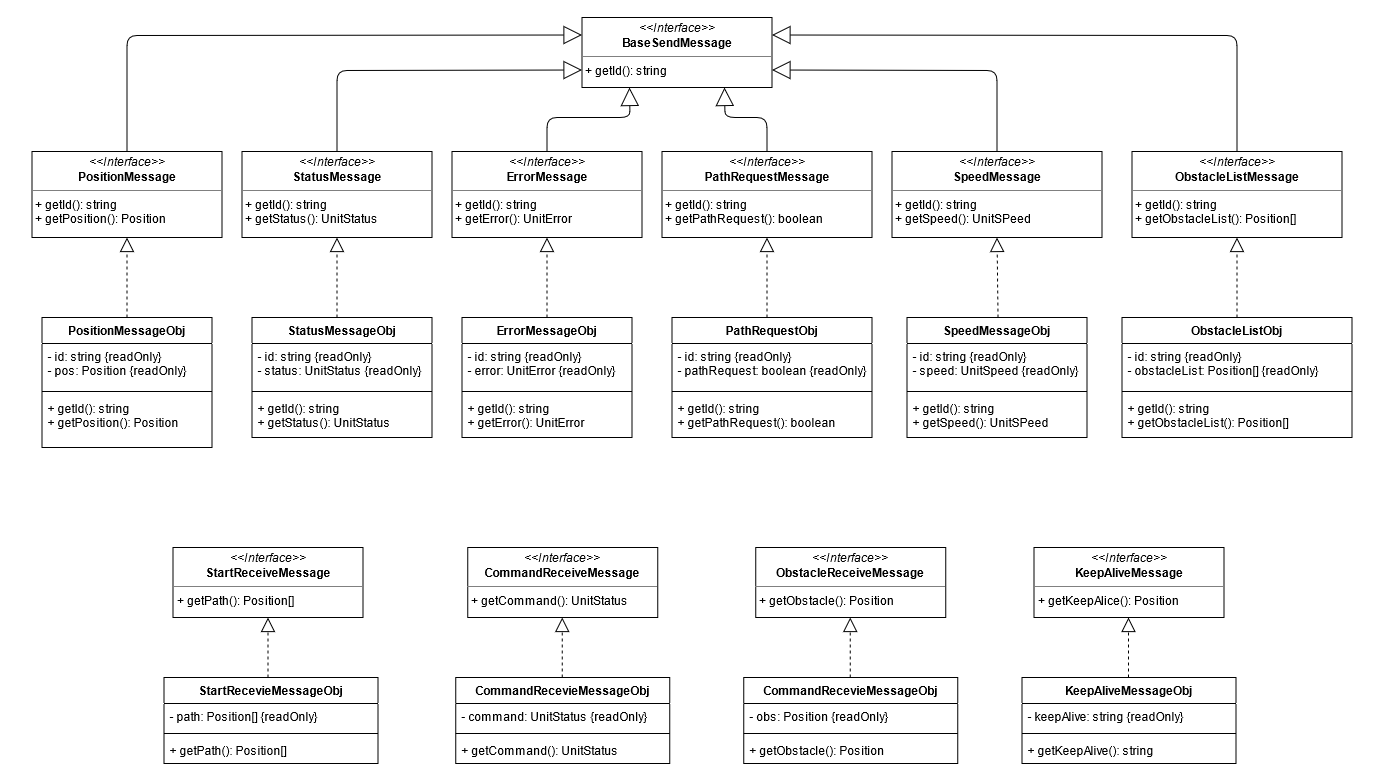
\includegraphics[width=25.5cm]{img/unit_messaggi.png}
    	\caption{Unità - Messaggi}
    \end{figure}
\end{landscape}